\documentclass[12pt]{article} 

% --- Layout ---
\usepackage[a4paper, margin=1in]{geometry} 
\usepackage{parskip}  
\usepackage{setspace} 
\usepackage{graphicx}

\onehalfspacing       

% --- Font ---
\usepackage{lmodern}  
\usepackage[T1]{fontenc}

% --- Math Packages ---
\usepackage{mathtools}
\allowdisplaybreaks


\begin{document}

\title{\Huge Newton-Euler Method}
\author{Jerry Wu}
\date{}
\maketitle

\begin{figure}[h]
    \centering
    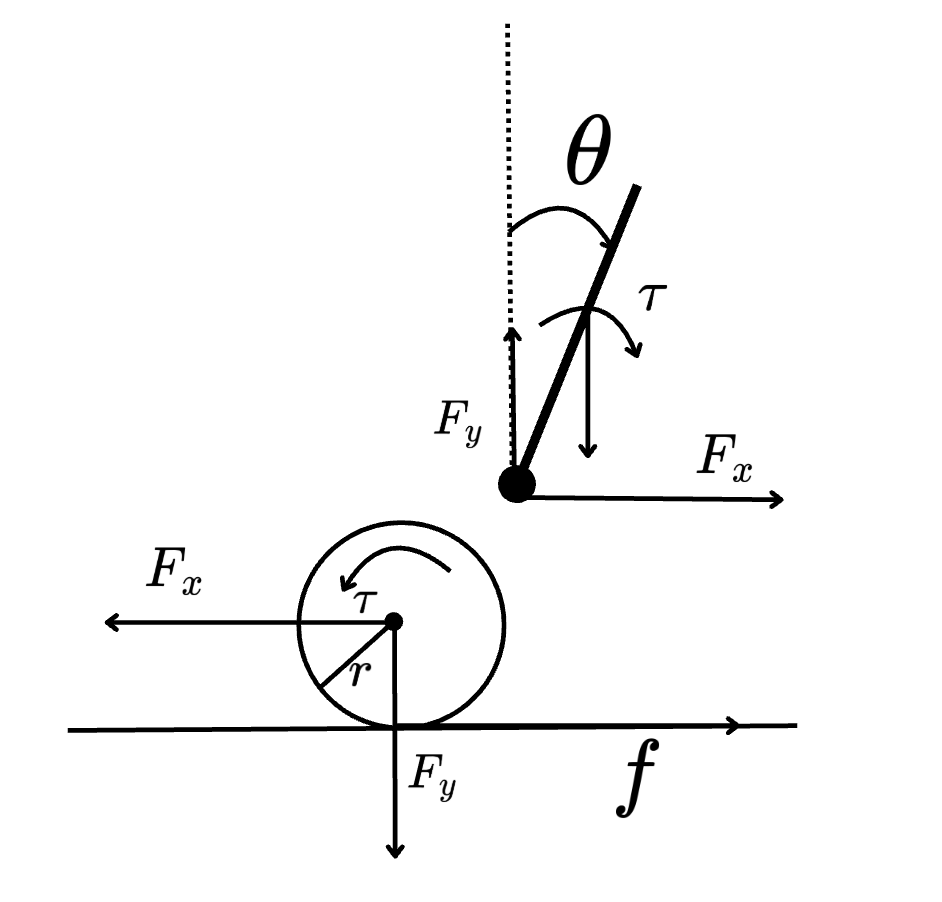
\includegraphics[width=0.5\textwidth]{Newton_Euler_Diagram.png}
    \caption{Newton Euler Method Diagram}
    \label{fig:your-label}
\end{figure}

\section*{Newton Euler Equations}
\[
\left\{
\begin{aligned}
a_{bx} &= \frac{F_x}{m_b}\text{(1)} \\
a_{by} &= \frac{F_y - m_b g}{m_b} \text{(2)}\\
\ddot{\theta} &= \frac{F_y r_b \sin(\theta) - F_x r_b \cos(\theta) + \tau}{I_b}\text{(3)}
\end{aligned}
\right. \quad \text{(Body)}
\]


\[
\left\{
\begin{aligned}
a_{wx} &= \frac{f - F_x}{m_w}\text{(4)} \\
\beta_w &= \frac{-\tau - f r}{I_w}\text{(5)}
\end{aligned}
\right. \quad \text{(Wheel)}
\]

\[
\left\{
\begin{aligned}
a_{bx} + \dot{\theta}^2 r_b \sin(\theta) - \ddot{\theta} r_b \cos(\theta) &= a_{wx}\text{(6)} \\
a_{by} + \dot{\theta}^2 r_b \cos(\theta) - \ddot{\theta} r_b \sin(\theta) &= 0 \text{(7)}\\
a_{wx} &= \beta_w r\text{(8)}
\end{aligned}
\right. \quad \text{(Constraint)}
\]

\section*{Solve}
\[
a_{wx} = \frac{r(-fr - \tau)}{I_w} \quad \text{(from (5)(8))} \tag{9}
\]

\[
a_{wx} = \frac{r(-r(F_x+M_wa_{wx})-\tau)}{I_w}\text{(from (4)(9))} \tag{10}
\]

\begin{align}
a_{wx} &= \frac{F_x}{M_b} - r_b \ddot{\theta} \cos(\theta) + r_b \dot{\theta}^2 \sin(\theta)\text{(from (1)(6))} \tag{11} \\
0 &= \frac{F_y}{M_b} + r_b \ddot{\theta} \sin(\theta) + r_b \dot{\theta}^2 \cos(\theta) - g \text{(from (2)(7))}\tag{12}
\end{align}

\begin{align}
\ddot{\theta} = \frac{1}{I_b} \Big[ 
    & r_b M_b \left( 
        -r_b \ddot{\theta} \sin(\theta) 
        - r_b \dot{\theta}^2 \cos(\theta) 
        + g 
    \right) \sin(\theta) \notag \\
    & - r_b M_b \left( 
        r_b \ddot{\theta} \cos(\theta) 
        - r_b \dot{\theta}^2 \sin(\theta) 
        + a_{wx} 
    \right) \cos(\theta) 
    + \tau 
\Big] 
\tag{14}
\end{align}

\[
a_{wx} = \ddot{x} = \frac{1}{I_w}{r \left( 
    -r \left( 
        M_b \left( 
            r_b \ddot{\theta} \cos(\theta) 
            - r_b \dot{\theta}^2 \sin(\theta) 
            + a_{wx} 
        \right) 
        + M_w a_{wx} 
    \right) 
    - \tau 
\right)}
\tag{15}
\]

\[
D = I_b I_w + I_b M_b r^2 + I_b M_w r^2 + I_w M_b r_b^2 + M_b^2 r^2 r_b^2 \sin^2(\theta) + M_b M_w r^2 r_b^2
\tag{16}
\]


\begin{align}
\ddot{x} = \frac{r}{D} \Big( 
    & I_b M_b \dot{\theta}^2 r r_b \sin(\theta)
    - I_b \tau 
    + M_b^2 \dot{\theta}^2 r r_b^3 \sin(\theta) \notag \\
    & - \frac{1}{2} M_b^2 g r r_b^2 \sin(2\theta)
    - M_b r r_b \tau \cos(\theta)
    - M_b r_b^2 \tau 
\Big)
\tag{17}
\end{align}

\begin{align}
\ddot{\theta} = \frac{1}{D} \Big( 
    & I_w M_b g r_b \sin(\theta)
    + I_w \tau 
    - \frac{1}{2} M_b^2 \dot{\theta}^2 r^2 r_b^2 \sin(2\theta) \notag \\
    & + M_b^2 g r^2 r_b \sin(\theta)
    + M_b M_w g r^2 r_b \sin(\theta) \notag \\
    & + M_b r^2 \tau
    + M_b r r_b \tau \cos(\theta)
    + M_w r^2 \tau 
\Big)
\tag{18}
\end{align}



\section*{Linearized System}
\[
\mathbf{A} =
\begin{bmatrix}
0 & 1 & 0 & 0 \\
0 & 0 & -\dfrac{M_b^2 g r^2 r_b^2}{D} & 0 \\
0 & 0 & 0 & 1 \\
0 & 0 & \dfrac{I_w M_b g r_b + M_b^2 g r^2 r_b + M_b M_w g r^2 r_b}{D} & 0
\end{bmatrix}
\]
\[
\mathbf{B} =
\begin{bmatrix}
0 \\
\dfrac{r(-I_b - M_b r r_b - M_b r_b^2)}{D} \\
0 \\
\dfrac{I_w + M_b r^2 + M_b r r_b + M_w r^2}{D}
\end{bmatrix}
\]
\[
D = I_b I_w + I_b M_b r^2 + I_b M_w r^2 + I_w M_b r_b^2 + M_b M_w r^2 r_b^2
\]



\end{document}